\documentclass[12pt,oneside,a4paper,english]{article}
\usepackage[T1]{fontenc}
\usepackage[utf8]{inputenc} % Changed from latin2 to utf8 for better compatibility
\usepackage[margin=2.25cm,headheight=26pt,includeheadfoot]{geometry}
\usepackage[english]{babel}
\usepackage{listings}
\usepackage{color}
\usepackage{titlesec}
\usepackage{titling}
\usepackage[framed, numbered]{matlab-prettifier}
\usepackage{changepage}
\usepackage{amsmath}
\usepackage{hyperref}
\usepackage{enumitem}
\usepackage{graphicx}
\usepackage{fancyhdr}
\usepackage{lastpage}
\usepackage{caption}
\usepackage{tocloft}
\usepackage{setspace}
\usepackage{multirow}
\usepackage{titling}
\usepackage{float}
\usepackage{comment}
\usepackage{booktabs}
\usepackage{indentfirst}
\usepackage{lscape}
\usepackage{booktabs,caption}
\usepackage[flushleft]{threeparttable}
\usepackage[english]{nomencl}
\usepackage{xcolor}
\usepackage{lipsum}

% Set up hyperref
\hypersetup{
    colorlinks=true,
    linkcolor=blue,
    filecolor=magenta,      
    urlcolor=cyan,
    pdftitle={Aldebaran Transit Near Venus in 2025},
    pdfpagemode=FullScreen,
}

% --- set footer and header ---
\pagestyle{fancy}
\fancyhf{}
\rhead{Review of }
\lhead{Astronomical Observation}
\rfoot{Page \thepage\ of \pageref{LastPage}}

% --- Title formatting ---
\title{\textbf{Aldebaran Transit Near Venus in 2025}}
\author{Astronomy Enthusiast}
\date{\today}

% --- Fix typo in Aldebaran throughout document ---
\newcommand{\Aldebaran}{Aldebaran}

% --- End of page settings ---
\begin{document}
\maketitle

\begin{abstract}
    This document will give an insight into the relationship of the Sun, Earth and Moon. To summarize, the sun is the center of our solar system and the Earth of orbiting around the sun. At the same time, the moon orbits around the Earth. These bodies are moving in a symphony of celestial mechanics, there is only a singular force that dictates this relationship. Gravity mediates our solar system and dictates the movements of the planets, moons and smaller orbiting bodies, the solar system began in a cloud of gas and dust, which collapsed under its own gravity. Forming our infant sun! This is where the story of our solar system and Earth began.
\end{abstract}
\section{Sun's Formation}
Newton's law of universal graviation describes the gravitational force between two objects as:
\begin{equation}
    F = \frac{G \cdot m_1 \cdot m_2}{r^2}
\end{equation}
Where $m_1$ and $m_2$ are the masses of the two objects, $r$ is the distance between their centers, and $G$ is the gravitational constant($6.674\cdot 10^{-11} m^3 \cdot kg^{-1} \cdot s^{-2}$). When one body is signicantly larger than the other body, gravity only really depends on the much more massive object, that is why on Earth gravity is understood as:
\begin{equation}
    F = \frac{G \cdot m_e}{r^2}
\end{equation}
The force of gravity is what keeps the planets in orbit around the sun and the moons in orbit around their respective planets. The sun's mass is so large that it creates a gravitational pull that keeps all of the planets in our solar system in orbit around it. This applies to smaller objects too! 4.6 billion years ago, the sun was a nebula of gas and dust particles. These dust particles attract one another and begin to clump together. As the particles clump together, they create larger and larger objects, this was called accretion. 
\begin{figure}[H]
    \centering
    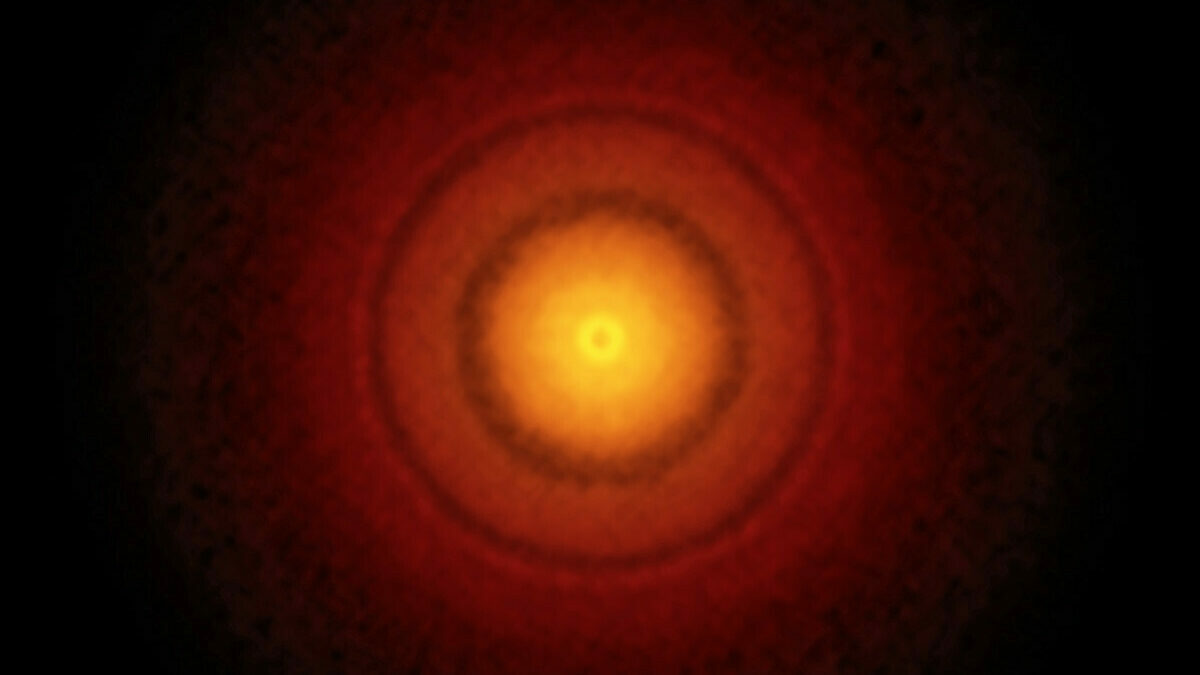
\includegraphics[width=0.5\textwidth]{SolarSys1.jpg}
    \caption{Image of an accretion disk of a new faraway Protostar, notice the small dark bands! These are paths of planets forming in the dust clouds.\cite{solarsysImg}}
    \label{fig:solardisk}
\end{figure}
The dust of this nebula is mostly hydrogen, helium, and a very microscopic fraction of all of the other elements. The accretion disk will begin to produce heat as they rub together and spin until the Protostar begins emitting light from this friction, there is no fusion yet. This star is still going to pull more materials into itself and while it is growing, planets and moons will also form via accretion. These bodies will not become larger enough for fusion to occur making them cooler than a star, all of these bodies will orbit the Protostar pulling in materials from their surroundings until the star begins to undergo fusion of hydrogen, once this begins the star will eject all of the dust immediately around the sun and becomes a main sequence star. This is still a turbulent time for the young sun and it's solar system, these planets and planet like objects known as planetismals were still colliding with each other and flinging debris into more chaotic orbits around the sun. The chaotic period after formation, was when the Earth collided with another proto planet named Theia\cite{moonformation}. This collision eventually made the body that would become our moon!
\section{The Earth and It's Moon}
The Earth or it's protoplanet formed beginnning 4.54 billion years ago as the protoplanent's accretion disk attracted enough material to collapse into roughly sphereical shape until the sun begin fusion ejecting all of the dust not held onto by Earth. All of the planets and planetismals around the Earth have orbits that are very close and will collide with Earth. The Earth would be in a cosmic game of bumper cars, sometimes the Earth would gain material from absorbing the body, or if the body was bigger that the Earth(or similar size to Earth), it would lose material. The Earth's surface would become very hot and molten, as the crust of the Earth and it's mantle cooled, the collision with Theia would have occurred and ejected some of the mantle and Theia's mantle into space. This debris was within the influence of Earth's gravity and began to orbit the Earth. Once the solar system began to calm down, the moon and Earth's surface would cool. 

The Earth and Moon are made of the same material, the Moon is a part of the Earth that was ejected into space. Why does the Moon not have an atmosphere like the Earth? This is because of the lack of atmosphere and the iron core of the Moon is much weaker making the Moons magentic field too small to prevent the sun plasma ejections or Solar Wind from stripping the Moon of it's atmosphere. The Earth has a much larger iron core and a much larger magnetic field, this is what protects the Earth from the solar wind. The moon is roughly a quarter the size of the Earth, and is 1/6th the gravity of the Earth. Now that the Earth and Moon exist together, they come togerther to form a graviational system we will call the Earth-Moon system, and this system revolves around the sun in its shared orbit. 

\section{References}
\bibliography{AstroTools.bib}
\bibliographystyle{ieeetr}
\end{document}

\end{document}